%% This is an example first chapter.  You should put chapter/appendix that you
%% write into a separate file, and add a line \include{yourfilename} to
%% main.tex, where `yourfilename.tex' is the name of the chapter/appendix file.
%% You can process specific files by typing their names in at the 
%% \files=
%% prompt when you run the file main.tex through LaTeX.
\chapter{Introduction}

\section{Section}\label{sec}

\subsection{Subsection}

Footnote\footnote{Here is a footnote}.
Refer to a section: section~\ref{sec}.
Refer to a figure: figure~\ref{rmse}.
Refer to a table: table~\ref{mytable}.
Cite a paper\cite{chien2002dynamic}.

%\lstset{language=Julia}
\begin{lstlisting}
print("hello world")
\end{lstlisting}

Example list
\begin{enumerate}
  \item Item 1
  \item Item 2
\end{enumerate}

Equation list
\begin{eqnarray*}
a_i & = & a_j + a_k \\
a_i & = & a_j \ll m \mbox{shift}
\end{eqnarray*}

%\nocite{key}

\begin{figure}
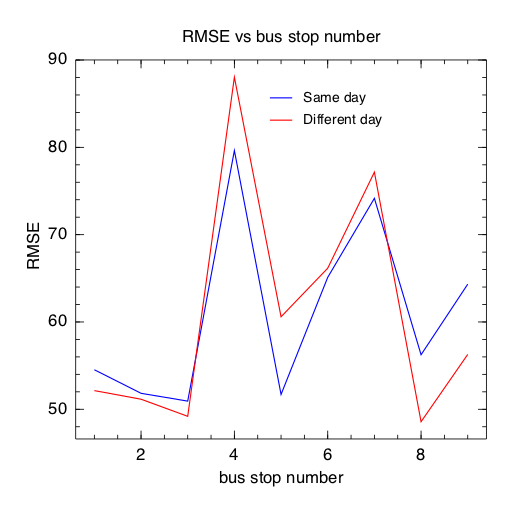
\includegraphics[width=\linewidth]{images/RMSEs.png}
%\vspace{2.4in}
\caption{RMSE}
\label{rmse}
\end{figure}
\clearpage
\newpage

\begin{table}
\caption{Table}
\label{mytable}
\begin{center}
\begin{tabular}{|l|l|}\hline
this & is \\\hline
a & table \\\hline
\end{tabular}
\end{center}
\end{table}

\clearpage
\newpage
